% ---
% Reemplaza líneas 2771–2841 de Docs/Technical_Report.tex.
% Decisiones que lo respaldan: D-013, D-014, D-015, D-016, D-017, D-027, D-030,
% D-031, D-035, H-012, H-019, H-031, H-034, H-053.
% ---

\subsection{Módulo 5: Transformación}
\label{sec:modulo5}

El módulo de transformación implementa las cinco condiciones experimentales del estudio. Todas
parten del mismo vector $\mathbf{x} \in [0,\pi]^{12}$ producido por M4 y su salida alimenta en
paralelo dos módulos independientes: el análisis de separabilidad (M6) y la clasificación (M7).
La Tabla~\ref{tab:condiciones} resume las cinco condiciones.

\begin{table}[H]
\centering
\caption{Cinco condiciones experimentales del Módulo 5}
\label{tab:condiciones}
\renewcommand{\arraystretch}{1.3}
\begin{tabularx}{\textwidth}{@{}llXl@{}}
\toprule
\textbf{ID} & \textbf{Nombre} &
\textbf{Transformación} & \textbf{Tipo} \\
\midrule
C1 & Sin transformación & El vector $\mathbf{x}$ pasa directamente al clasificador. & Clásico \\
C2 & PCA lineal & Proyección sobre las 12 componentes principales. Es una rotación,
     así que actúa como control nulo. & Clásico \\
C3 & Kernel PCA (RBF) & Proyección no lineal a 12 dimensiones con kernel gaussiano;
     $\gamma$ por la heurística de la mediana. & Clásico \\
C4 & \texttt{zz\_feature\_map} & Primer orden en $Z$ y acoplamiento $ZZ$, seguidos de
     \texttt{real\_amplitudes} con $\boldsymbol\theta$ fijo. Salida:
     $\langle Z_i\rangle\in[-1,1]^{12}$. & Cuántico \\
C5 & \texttt{pauli\_feature\_map}$(Y, ZZ)$ & Primer orden en $Y$ y el mismo acoplamiento $ZZ$,
     con el mismo \textit{ansatz} y $\boldsymbol\theta$. Salida:
     $\langle Z_i\rangle\in[-1,1]^{12}$. & Cuántico \\
\bottomrule
\end{tabularx}
\end{table}

\textbf{Sobre la condición C2.} Dado que M4 entrega un vector ya de dimensión $k=12$, una
proyección PCA a 12 componentes no constituye una reducción de dimensionalidad sino una
rotación ortogonal, que preserva las distancias euclidianas. En consecuencia, los índices
de Davies-Bouldin y Fisher y el \textit{kernel-target alignment} son invariantes ante ella,
y el perceptrón absorbe la rotación en su primera capa lineal. C2 se conserva
deliberadamente como \textbf{control nulo}: si las métricas de separabilidad arrojaran
valores distintos para C1 y C2, ello indicaría un defecto en su implementación. El
comparador clásico sustantivo es C3.

% fuente: H-045; X4_67_features.csv. Entrelazamiento completo verificado el 2026-10-15:
% zz_feature_map(12, reps=1) y pauli_feature_map(12, reps=1, paulis=['Y','ZZ']) tienen 132 CNOT (66 pares).
% respaldo: «We identify four sources that can lead to concentration including expressivity of data embedding, global measurements, entanglement and noise.» (Thanasilp2024, p. 1)
% respaldo: «Repeating an encoding gate can help to increase the frequency spectrum, and thereby the expressivity of a quantum model.» (Schuld2021Encoding, p. 10)
% respaldo: «We introduce a class of quantum kernels that can be used for data with a group structure.» (Glick2024Covariant, p. 1)
\textbf{Por qué mapas con entrelazamiento.} Las dos condiciones cuánticas usan mapas de una
misma familia, con acoplamiento $ZZ$ entre todos los pares de qubits: 66 pares con $k = 12$. Se
descartaron como condiciones la codificación angular producto, sin entrelazamiento, y la
codificación en amplitudes, porque el kernel de ambas equivale por construcción a un kernel clásico. En la codificación angular, cada característica gira su propio qubit y el estado
es un producto, $|\phi(\mathbf{x})\rangle = \bigotimes_{i=1}^{k} R_Y(x_i)|0\rangle$. Su fidelidad
se factoriza en
\begin{equation}
  K(\mathbf{x},\mathbf{x}') = \prod_{i=1}^{k} \cos^2\!\left(\frac{x_i - x'_i}{2}\right),
  \label{eq:kernel_angular}
\end{equation}
que se calcula con $k$ operaciones clásicas y que, para diferencias pequeñas, se aproxima a un
kernel gaussiano. En la codificación en amplitudes, el kernel es el cuadrado de la similitud
coseno entre los vectores, un kernel polinomial clásico. Ambas equivalencias se comprobaron
numéricamente en los experimentos complementarios
(sección~\ref{sec:experimentos_complementarios}). Ninguna de las dos codificaciones podría, por
tanto, mostrar una separabilidad que no ofrezcan ya los métodos clásicos.

El entrelazamiento cambia esto. El acoplamiento $ZZ$ añade a cada par de qubits una fase que
depende del producto $(\pi - x_i)(\pi - x_j)$, y el estado deja de ser un producto de estados
de un qubit: la fidelidad ya no se descompone en contribuciones independientes por
característica, y el kernel incorpora interacciones entre pares de características que la
ecuación~\eqref{eq:kernel_angular} no puede expresar. Esa es la condición mínima para que la
pregunta de investigación no tenga respuesta de antemano, no una garantía de mejora: el
entrelazamiento figura también entre las fuentes de concentración de los kernels cuánticos que
identifican Thanasilp et al. \cite{Thanasilp2024}, y la concentración observada en C4 y C5 se
cuantifica en el capítulo~\ref{sec:resultados}. Otras familias con entrelazamiento quedaron fuera
por el propio diseño. Los circuitos que repiten la codificación intercalada con capas
entrenables, cuya expresividad estudian Schuld et al. \cite{Schuld2021Encoding}, requieren
entrenar parámetros, y aquí $\boldsymbol\theta$ se mantiene fijo. Los kernels covariantes de Glick
et al. \cite{Glick2024Covariant} están pensados para datos con estructura de grupo, que las
características radiómicas no tienen.

\textbf{Sobre la elección de C5.} La biblioteca Qiskit define \texttt{ZZFeatureMap} como un
caso particular de \texttt{PauliFeatureMap} con operadores $(Z, ZZ)$; ambas construcciones
preparan el mismo estado, con fidelidad $|\langle\phi_{ZZ}|\phi_{\text{Pauli}}\rangle|^2 = 1$.
Especificadas así, C4 y C5 no constituirían condiciones independientes. Se consideró
primero el conjunto $(X, ZZ)$, pero con una repetición el término en $X$ actúa sobre el
estado $|+\rangle$ que deja la capa de Hadamard, que es autoestado de $X$, y solo añade
una fase global: C5 equivaldría a un \textit{feature map} con únicamente el acoplamiento
$ZZ$. Se adopta por tanto el conjunto $(Y, ZZ)$. Sobre la esfera de Bloch, el giro en
$Z$ de C4 desplaza cada qubit a lo largo del ecuador y solo cambia una fase relativa,
mientras que el giro en $Y$ de C5 lo saca del ecuador y cambia las probabilidades de medir
0 y 1. Ambas condiciones comparten el acoplamiento $ZZ$ y el número de compuertas de
entrelazamiento, de modo que la comparación entre C4 y C5 mide el efecto del eje de la
codificación de primer orden.

Los parámetros $\boldsymbol\theta$ del \textit{ansatz} \texttt{real\_amplitudes}, 24 en total con
una repetición, se fijan una sola vez con una semilla declarada (42), muestreados de manera
uniforme en $[0,2\pi)$, y no se entrenan. Los valores esperados $\langle Z_i\rangle$ se calculan de
forma exacta a partir del vector de estado, una sola vez para todo el conjunto, y se guardan en
disco. En el resto del reporte este diseño se denomina \emph{Arquitectura~B}: el circuito actúa como
extractor fijo y solo se entrena el MLP sobre los valores guardados. La alternativa descartada,
\emph{Arquitectura~A}, entrenaría $\boldsymbol\theta$ junto con el MLP, extremo a extremo, y exigiría
evaluar el circuito y su gradiente en cada época.
% Añadido el 2026-10-19 (auditoría A5-10): «Arquitectura A/B» se usaba en §5.11, §6.7, §6.8 y §8.1 sin definirse.
El \textit{ansatz} no puede suprimirse. En C4, el \textit{feature map} aplica compuertas de Hadamard
seguidas de compuertas diagonales, que cambian las fases de las amplitudes pero no sus magnitudes.
Partiendo de $H^{\otimes k}|0\rangle$, toda amplitud conserva la magnitud $2^{-k/2}$, de modo que
$P(q_i = 0) = 1/2$ y $\langle Z_i\rangle = 0$ para cualquier entrada. La información codificada
reside en las fases, a las que una medición en la base $Z$ es insensible, y el \textit{ansatz} es lo
que las convierte en probabilidades medibles. En C5 el giro en $Y$ sí cambia las probabilidades, pero
sin el \textit{ansatz} $\langle Z_i\rangle = -\sin(2x_i)$ dependería de una sola característica y las
fases del acoplamiento $ZZ$ seguirían sin verse.

Además de los \textit{embeddings}, para C4 y C5 se calcula, con el \textit{feature map} solo,
el kernel de fidelidad
$K_Q(\mathbf{x},\mathbf{x}') = |\langle\phi(\mathbf{x})|\phi(\mathbf{x}')\rangle|^2$. El \textit{ansatz} no interviene, porque un mismo unitario aplicado a
ambos estados no cambia su producto interno. Este kernel es la entrada del análisis de
separabilidad (M6).

Ambos circuitos tienen 12 qubits y una repetición del \textit{feature map}, y comparten las mismas
compuertas de entrelazamiento. C5 solo añade las compuertas que realizan el giro en $Y$.

\begin{figure}[htbp]
\centering
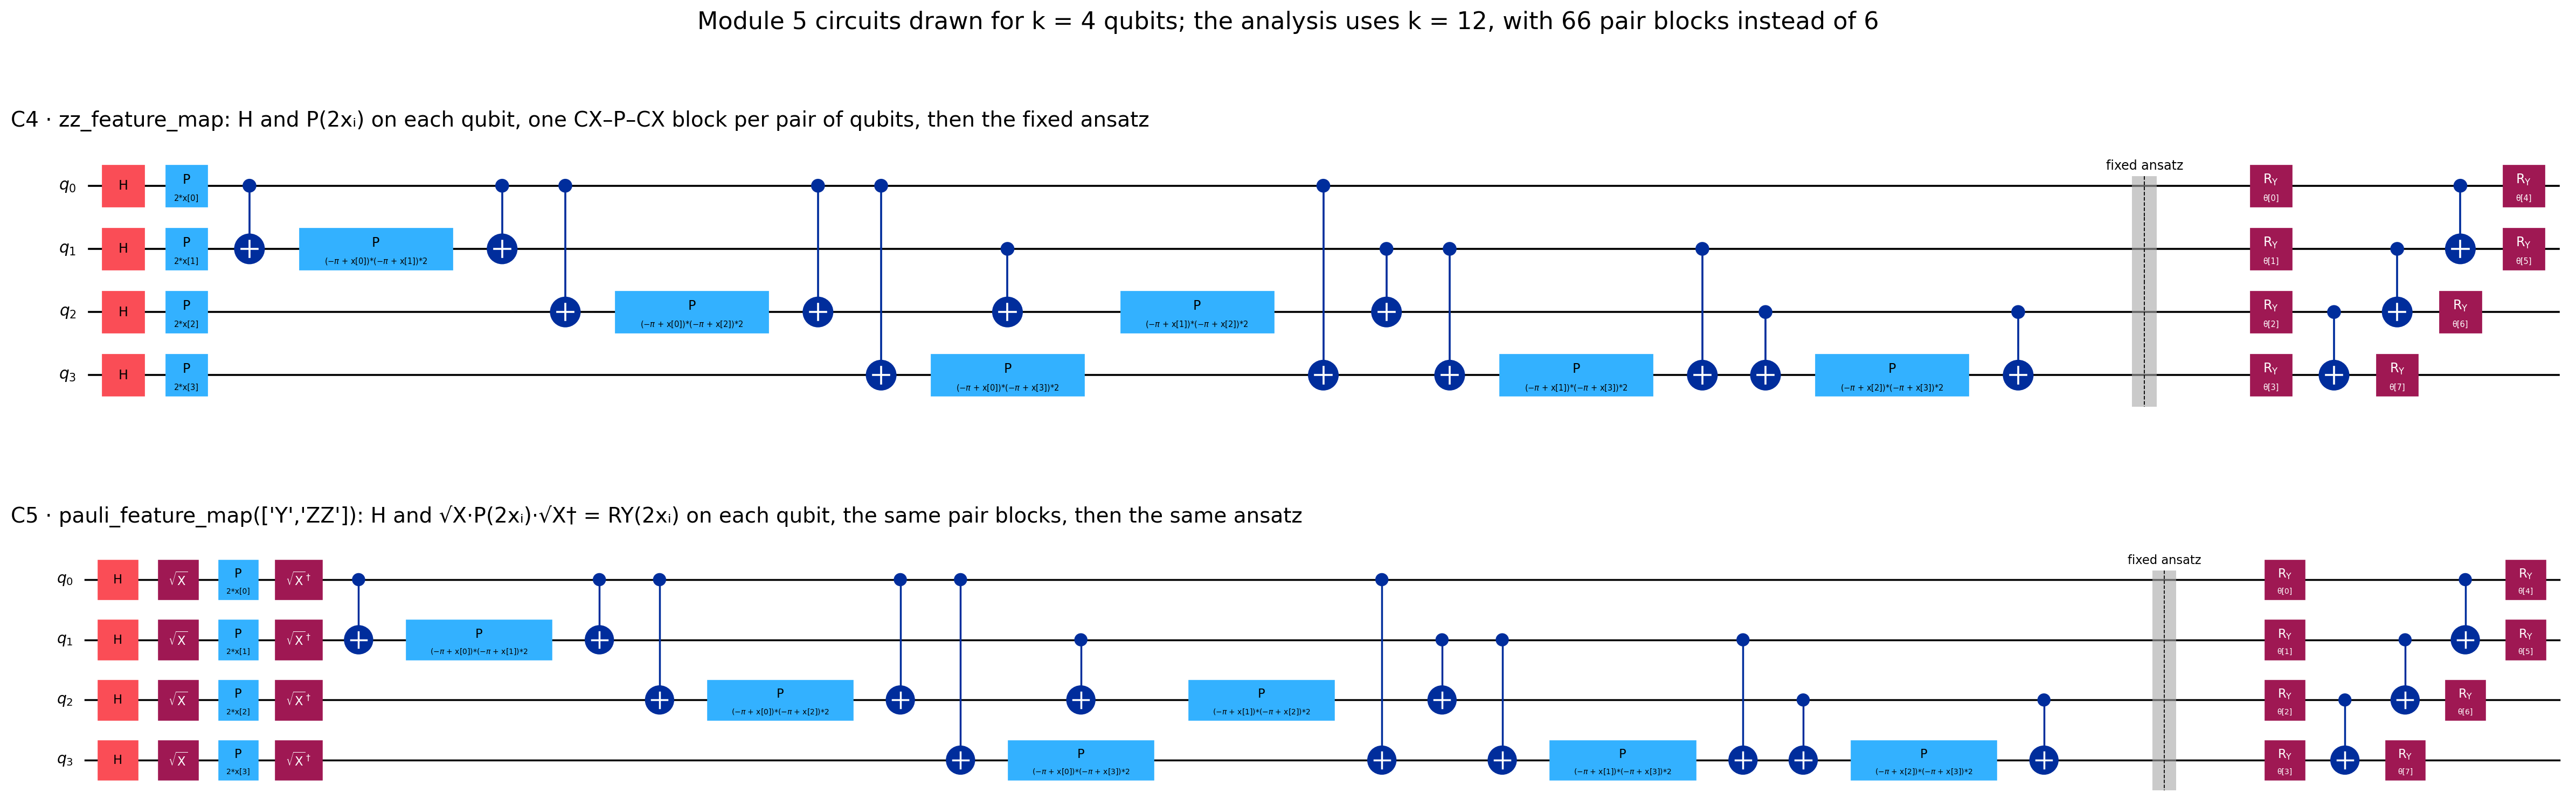
\includegraphics[width=\textwidth]{Figures/M5_circuit_k4.png}
\caption{Circuitos de C4 y C5 dibujados para $k=4$; el análisis usa $k=12$, con 66 bloques de pares en lugar de 6; la barrera separa el \textit{feature map} del \textit{ansatz} fijo.}
\label{fig:circuitos_k4}
\end{figure}
